\documentclass[11pt,a4paper]{article}
\usepackage[utf8]{inputenc}
\usepackage[T1]{fontenc}
\usepackage[french]{babel}
\usepackage{lmodern,microtype}
\usepackage[margin=2.05cm]{geometry}
\usepackage{amsmath,amssymb,booktabs,tabularx,longtable,graphicx,xcolor,hyperref,float,enumitem}
\definecolor{blueNG}{HTML}{174A70}
\hypersetup{colorlinks=true,linkcolor=blueNG,urlcolor=blueNG,pdftitle={Expérience NGeGenBrain : sondes adaptatives et neurones}}
\graphicspath{{figures/}}
\title{\vspace{-1cm}\textcolor{blueNG}{\bfseries Expérience NGeGenBrain : sondes adaptatives et neurones artificiels}\\[.2em]\large Rapport scientifique complet — exécution confirmatoire et analyses complémentaires}
\author{Dossier expérimental NGeGenBrain}
\date{28 octobre 2026}
\begin{document}\maketitle
\begin{abstract}
Ce travail compare des sondes RBF adaptatives, une variante dont les taux d'adaptation sont méta-appris, une sonde RBF fixe et un MLP de référence sur trois tâches synthétiques et deux benchmarks réels compacts : diagnostic binaire et chiffres manuscrits à dix classes. Il mesure en parallèle l'imitation en boîte noire de neuf neurones artificiels isolés, puis remplace progressivement des neurones cachés par des sondes dans deux compositions. Les résultats soutiennent une conclusion limitée : une sonde adaptative peut apprendre des tâches de classification et approximer certains neurones simples à partir d'observations autorisées ; la fidélité se dégrade sous changement de distribution et lors du remplacement de composants en composition. Ces expériences ne démontrent pas une équivalence générale entre neurones et sondes.
\end{abstract}
\tableofcontents\newpage
\section{Résumé exécutif et verdict}
L'expérience demandée est une étude de la relation entre une sonde adaptative et un neurone, pas une reconstruction de LLM. Elle comporte trois parties complémentaires : apprentissage d'une tâche avec quatre méthodes, imitation de neurones artificiels observés uniquement par leurs entrées/sorties, et composition de sondes en remplacement d'unités cachées d'un réseau source.

\begin{itemize}[leftmargin=1.2cm]
\item \textbf{Classification.} Les sondes adaptatives sont compétitives sur les quatre tâches. La variante à taux d'adaptation méta-appris obtient la meilleure exactitude moyenne sur deux lunes, cercles et cancer du sein ; sur le produit/XOR bruité, elle est comparable aux autres méthodes. Le contrôle fixe est inférieur sur les tâches considérées, mais son nombre de paramètres entraînables est inférieur (17 contre 65 en 2D ou 513 en 30D, et 170 contre 1 210 sur les chiffres) : cette comparaison ne sépare donc pas entièrement adaptation et capacité. Le complément réel à dix classes montre aussi que la RBF adaptative (87.31\%) reste sous le MLP (96.76\%) et que B à taux méta-appris (78.33\%) n'améliore pas A.
\item \textbf{Imitation isolée.} Avec 256 paires, les sondes RBF à 81 paramètres donnent sur des entrées tenues à part un RMSE moyen d'environ 0.102 sur ReLU, 0.021 sur sigmoïde et 0.050 sur tanh. Le résultat montre l'approximation de neurones simples sur un domaine précis ; il ne prouve pas leur équivalence générale. Les sensibilités au budget de paramètres et au décalage d'entrée sont importantes.
\item \textbf{Composition.} Le remplacement de 16 unités dans un MLP à 16 unités cachées accroît l'écart de logits moyen jusqu'à environ 0.45 sur deux lunes et 1.44 sur le benchmark réel. L'exactitude peut rester stable ou même augmenter sans que les sorties soient fidèles au modèle source.
\item \textbf{Intégrité.} L'audit du jeu de données retrouve zéro chevauchement de hachages de lignes entre train/validation/test pour chaque partition, et les interfaces d'ajustement ne prennent pas les labels de test en arguments. Le statut est \texttt{PASS\_WITH\_LIMITATIONS} : l'environnement n'est pas un bac à sable OS adversarial, et l'audit de flux de données n'est pas une preuve absolue d'absence de tout canal caché.
\end{itemize}

\section{Analyse des documents sources}
\subsection{Formalisation NGeGenBrain \texttt{full\_0}}
La définition utilisée indique qu'une sonde est un opérateur d'observation identifié et versionné, avec domaine, codomaine, procédure d'acquisition, préconditions, budget/coût, niveau d'intrusion, sérialisation et contrôle. L'application d'observation est représentée par $\Phi(p,x,f)\in Y_f$. La théorie insiste aussi sur le contexte, les transformations déclarées, la distinction entre empreinte et dossier d'évidence, et la condition d'injectivité pour une reconstruction exacte. Elle ne définit pas, à elle seule, une sonde comme un réseau apprenant ou comme un neurone.

L'extension de ce rapport est explicitement additive : une sonde paramétrée $P_\theta$ adapte ses paramètres selon un signal admissible ; une variante méta-apprend des taux de mise à jour ; une sonde imitatrice apprend une fonction cible uniquement à partir de couples observés $(x,N(x))$. Les définitions et limites sont détaillées dans \texttt{formalisme\_sonde\_adaptative.tex}.

\subsection{Expérience antérieure sur deux lunes}
Le rapport antérieur comparait 12 sondes RBF adaptatives, un MLP et des sondes fixes sur une seule tâche synthétique, avec cinq initialisations. Il annonçait 96.005\% pour les RBF adaptatives, 95.870\% pour le MLP, et 86.230\% pour le contrôle fixe. Ce résultat motivait le suivi, mais ne testait ni l'imitation de neurones ni la composition. Il est conservé comme contexte historique, pas combiné aux nouvelles mesures.

\section{Hypothèses et conditions expérimentales}
Les hypothèses opérationnelles sont : (H1) une sonde adaptative peut apprendre une tâche ; (H2) une sonde peut approximer l'entrée-sortie d'un neurone sans connaître ses paramètres ; (H3) la fidélité peut tenir sur entrées indépendantes ; (H4) des sondes substituées se composent avec une dégradation mesurable ; (H5) les résultats varient selon tâches, budgets et domaine ; (H6) il faut distinguer rôle observationnel, approximation empirique et équivalence mathématique.

Les conditions comparées sont :
\begin{enumerate}[leftmargin=1.1cm]
\item A — RBF adaptative, paramètres ajustés par Adam sur les labels autorisés ;
\item B — même famille RBF, taux d'actualisation par groupe méta-appris par hypergradient sur train/validation ;
\item contrôle — centres et largeurs RBF fixes, lecture entraînable seulement ;
\item D — MLP de référence à 16 unités tanh ;
\item C1 — imitation entrée-sortie de neuf neurones simples à poids cachés ;
\item C2 — imitation de 16 activations cachées, puis remplacement de 1, 4 ou 16 composants dans deux MLP.
\end{enumerate}

\section{Protocole, données et règle rouge}
\subsection{Tâches}
Trois tâches synthétiques sont générées de manière déterministe : deux lunes, cercles concentriques et classification du signe du produit $x_1x_2$ avec 4\% de bruit de label. Les cas réels sont le dataset public Wisconsin Diagnostic Breast Cancer fourni par scikit-learn (569 exemples, 30 variables) et, dans le complément préenregistré, le jeu de chiffres manuscrits scikit-learn (1 797 images 8×8, 64 variables, 10 classes). Ce sont des benchmarks compacts ; le premier n'est pas une validation clinique et le second n'est pas une validation en production.

\subsection{Partitions et paramètres}
Les données sont réparties stratifié en 60\% entraînement, 20\% validation et 20\% test. Les graines confirmatoires sont 714, 825 et 936. Le standardiseur n'est ajusté que sur train (60\%). Les modèles finaux de classification sont réajustés sur train+validation ; le jeu de test n'entre pas dans l'ajustement. Sur les données synthétiques, la partition compte 1080/360/360 exemples ; sur le benchmark réel, 341/114/114.

La sonde RBF de classification a 16 centres et exactement le même nombre de paramètres entraînables que le MLP correspondant : 65 en dimension 2 et 513 en dimension 30. Le contrôle fixe n'a que 17 paramètres entraînables. La condition B apprend quatre taux par groupe à partir d'épisodes de train/validation puis entraîne 700 époques ; A, le contrôle et le MLP sont entraînés 220 époques dans l'analyse principale. Pour traiter ce déséquilibre de budget, une analyse secondaire à 700 époques finales pour les quatre méthodes est rapportée séparément.

\subsection{Séparation des données et fuites}
Pour l'imitation isolée, la sonde reçoit uniquement les observations $(x_i,y_i)$ interrogées sur la cible. Ni la famille d'activation, ni la graine/les paramètres du neurone cible, ni les sorties de test ne sont des arguments de la fonction d'ajustement. Les graines des sondes (111, 222, 333) sont indépendantes des neuf graines des cibles (107, 110, 113, 208, 211, 214, 309, 312, 315). Pour la composition, les sondeurs reçoivent l'entrée et les activations cachées observées seulement sur train ; les activations de test servent à calculer les métriques une fois les sondes gelées.

L'audit recalcule les hachages des lignes brutes par tâche/partition et obtient zéro chevauchement de hachages entre train, validation et test, pour 17 907 enregistrements de partition. Les interfaces d'ajustement ont été inspectées et les prédictions sont reproductibles octet par octet lors d'une relance par étapes. Limite importante : l'exécution a lieu dans un orchestrateur local et non dans un bac à sable résistant à un processus hostile ayant accès arbitraire au système de fichiers ; aucune affirmation d'absence absolue de canaux cachés n'est faite.

Le protocole version 1.1 a été haché avant l'exécution confirmatoire indépendante. L'audit a détecté que la première composition utilisait par erreur les graines de classification 714/825/936 au lieu des graines de composition spécifiées 411/522/633. Ces lots déviants sont conservés sous audit, exclus des synthèses et remplacés par six lots exécutés après gel du correctif v1.2. Les analyses sur décalage de distribution, budget de paramètres et époques égales sont des extensions exploratoires ajoutées après l'analyse principale et identifiées comme telles.

\section{Résultats 1 — Apprentissage de tâches}
Les nombres sont des moyennes $\pm$ écarts-types sur trois partitions/graines distinctes. Le petit nombre de graines implique des intervalles de confiance larges ; il ne permet pas de déclarer une supériorité universelle.
\begin{table}[htbp]
\centering
\small
\setlength{\tabcolsep}{4pt}
\renewcommand{\arraystretch}{1.08}
\begin{tabular}{llrrrr}
\toprule
Méthode & Exactitude \% & F1 \% & ROC-AUC & Log-loss & Param. \\
\midrule
Sonde RBF fixe & 85.37 $\pm$ 1.16 & 85.21 $\pm$ 0.93 & 0.9260 $\pm$ 0.0060 & 0.351 $\pm$ 0.012 & 17 \\
Sonde RBF adaptative & 93.61 $\pm$ 0.56 & 93.59 $\pm$ 0.63 & 0.9794 $\pm$ 0.0045 & 0.204 $\pm$ 0.018 & 65 \\
Sonde à mécanisme partiellement appris & 95.74 $\pm$ 0.58 & 95.76 $\pm$ 0.55 & 0.9899 $\pm$ 0.0031 & 0.127 $\pm$ 0.010 & 65 \\
MLP de référence & 90.74 $\pm$ 2.52 & 90.67 $\pm$ 2.64 & 0.9673 $\pm$ 0.0184 & 0.233 $\pm$ 0.060 & 65 \\
\bottomrule
\end{tabular}
\caption{Classification sur Deux lunes. Moyenne $\pm$ écart-type sur trois partitions/graines distinctes. Les écarts-types de l'exactitude et du F1 sont en points de pourcentage.}
\label{tab:class_two_moons}
\end{table}
\begin{table}[htbp]
\centering
\small
\setlength{\tabcolsep}{4pt}
\renewcommand{\arraystretch}{1.08}
\begin{tabular}{llrrrr}
\toprule
Méthode & Exactitude \% & F1 \% & ROC-AUC & Log-loss & Param. \\
\midrule
Sonde RBF fixe & 90.56 $\pm$ 1.11 & 91.20 $\pm$ 0.95 & 0.9774 $\pm$ 0.0040 & 0.403 $\pm$ 0.034 & 17 \\
Sonde RBF adaptative & 94.35 $\pm$ 0.89 & 94.34 $\pm$ 0.88 & 0.9898 $\pm$ 0.0036 & 0.151 $\pm$ 0.015 & 65 \\
Sonde à mécanisme partiellement appris & 94.72 $\pm$ 1.11 & 94.72 $\pm$ 1.12 & 0.9901 $\pm$ 0.0034 & 0.130 $\pm$ 0.020 & 65 \\
MLP de référence & 94.44 $\pm$ 1.21 & 94.41 $\pm$ 1.20 & 0.9887 $\pm$ 0.0035 & 0.156 $\pm$ 0.017 & 65 \\
\bottomrule
\end{tabular}
\caption{Classification sur Cercles. Moyenne $\pm$ écart-type sur trois partitions/graines distinctes. Les écarts-types de l'exactitude et du F1 sont en points de pourcentage.}
\label{tab:class_circles}
\end{table}
\begin{table}[htbp]
\centering
\small
\setlength{\tabcolsep}{4pt}
\renewcommand{\arraystretch}{1.08}
\begin{tabular}{llrrrr}
\toprule
Méthode & Exactitude \% & F1 \% & ROC-AUC & Log-loss & Param. \\
\midrule
Sonde RBF fixe & 91.85 $\pm$ 1.85 & 92.10 $\pm$ 1.71 & 0.9461 $\pm$ 0.0026 & 0.435 $\pm$ 0.007 & 17 \\
Sonde RBF adaptative & 94.17 $\pm$ 0.48 & 94.32 $\pm$ 0.41 & 0.9490 $\pm$ 0.0017 & 0.287 $\pm$ 0.005 & 65 \\
Sonde à mécanisme partiellement appris & 93.80 $\pm$ 1.12 & 93.97 $\pm$ 1.00 & 0.9487 $\pm$ 0.0016 & 0.280 $\pm$ 0.008 & 65 \\
MLP de référence & 94.26 $\pm$ 0.42 & 94.40 $\pm$ 0.33 & 0.9530 $\pm$ 0.0034 & 0.261 $\pm$ 0.006 & 65 \\
\bottomrule
\end{tabular}
\caption{Classification sur Produit/XOR bruité. Moyenne $\pm$ écart-type sur trois partitions/graines distinctes. Les écarts-types de l'exactitude et du F1 sont en points de pourcentage.}
\label{tab:class_xor_product}
\end{table}
\begin{table}[htbp]
\centering
\small
\setlength{\tabcolsep}{4pt}
\renewcommand{\arraystretch}{1.08}
\begin{tabular}{llrrrr}
\toprule
Méthode & Exactitude \% & F1 \% & ROC-AUC & Log-loss & Param. \\
\midrule
Sonde RBF fixe & 91.81 $\pm$ 1.34 & 93.73 $\pm$ 0.92 & 0.9821 $\pm$ 0.0121 & 0.244 $\pm$ 0.055 & 17 \\
Sonde RBF adaptative & 96.49 $\pm$ 1.52 & 97.25 $\pm$ 1.18 & 0.9942 $\pm$ 0.0070 & 0.132 $\pm$ 0.025 & 513 \\
Sonde à mécanisme partiellement appris & 98.25 $\pm$ 0.88 & 98.61 $\pm$ 0.70 & 0.9947 $\pm$ 0.0078 & 0.088 $\pm$ 0.034 & 513 \\
MLP de référence & 97.95 $\pm$ 1.01 & 98.38 $\pm$ 0.80 & 0.9926 $\pm$ 0.0078 & 0.087 $\pm$ 0.052 & 513 \\
\bottomrule
\end{tabular}
\caption{Classification sur Cancer du sein (benchmark). Moyenne $\pm$ écart-type sur trois partitions/graines distinctes. Les écarts-types de l'exactitude et du F1 sont en points de pourcentage.}
\label{tab:class_breast_cancer}
\end{table}
\begin{figure}[htbp]\centering
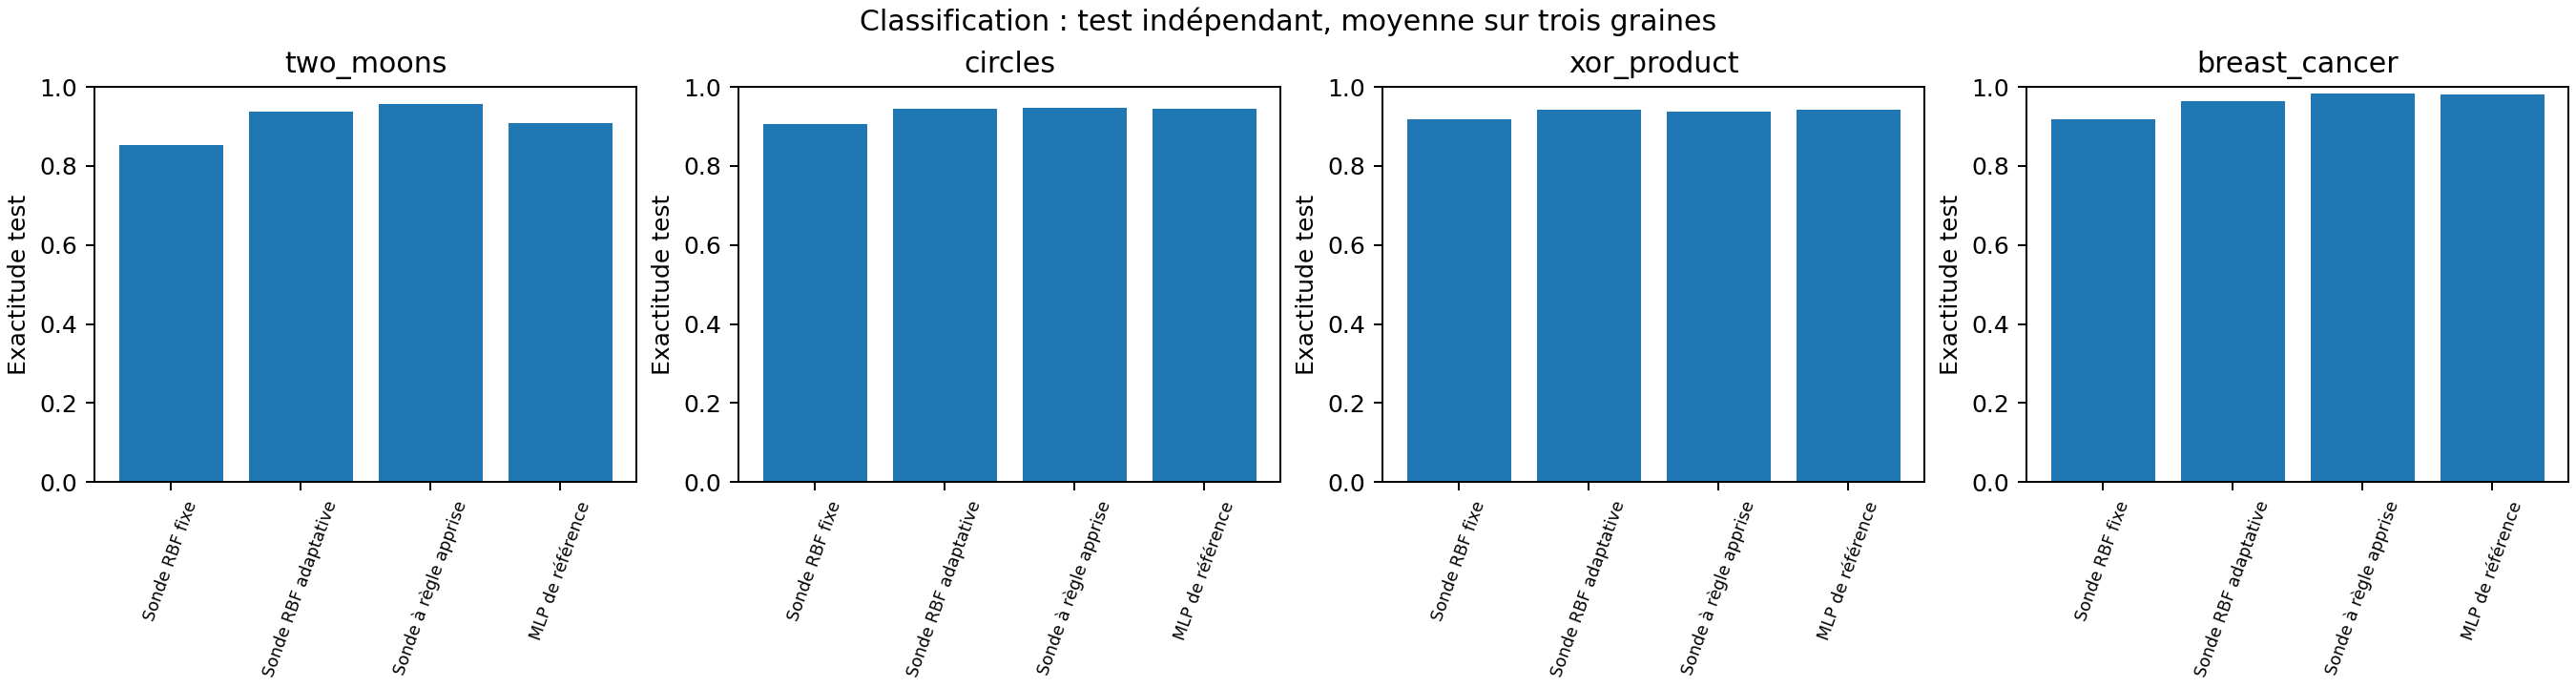
\includegraphics[width=.78\textwidth]{comparaison_classification.png}
\caption{Exactitude moyenne par tâche et méthode. Les trois graines sont montrées dans les tables précédentes ; le graphique synthétise seulement les tendances.}\label{fig:classification}
\end{figure}

\subsection{Lecture}
Sur deux lunes, B atteint environ 95.74\% d'exactitude contre 93.61\% pour A, 90.74\% pour le MLP et 85.37\% pour le contrôle fixe. Sur les cercles, les méthodes adaptatives sont très proches, tandis que la sonde fixe est plus faible. Sur le produit/XOR bruité, les quatre méthodes sont assez proches entre elles, avec le MLP à environ 94.26\%, A à 94.17\%, B à 93.80\% et la sonde fixe à 91.85\%. Sur le benchmark réel, B est à 98.25\%, le MLP à 97.95\%, A à 96.49\% et le contrôle fixe à 91.81\%.

Ces résultats soutiennent H1 : les sondes adaptatives apprennent bien ces tâches sous les budgets considérés. Les résultats du contrôle fixe sont compatibles avec l'utilité des degrés de liberté adaptatifs, mais le contrôle fixe a moins de paramètres, donc l'expérience n'isole pas parfaitement l'effet de l'adaptation.

\section{Résultats 2 — Imitation d'un neurone isolé}
Neuf neurones cibles boîte noire sont étudiés : trois avec activation tanh, trois ReLU et trois sigmoïde. Les sondes reçoivent 64, 256 ou 1024 paires de requêtes. Le test comporte 4000 entrées indépendantes dans la même distribution uniforme que l'apprentissage. L'activation cible est une métadonnée de l'évaluateur et n'est pas fournie à la fonction d'ajustement.

\begin{table}[htbp]
\centering
\small
\setlength{\tabcolsep}{4pt}
\renewcommand{\arraystretch}{1.08}
\begin{tabular}{llrrr}
\toprule
Activation cible (évaluateur seulement) & Paires observées & MAE & RMSE & R$^2$ \\
\midrule
tanh & 64 & 0.0482 $\pm$ 0.0312 & 0.0718 $\pm$ 0.0436 & 0.9898 $\pm$ 0.0081 \\
tanh & 256 & 0.0382 $\pm$ 0.0215 & 0.0501 $\pm$ 0.0264 & 0.9951 $\pm$ 0.0031 \\
tanh & 1024 & 0.0324 $\pm$ 0.0171 & 0.0427 $\pm$ 0.0218 & 0.9963 $\pm$ 0.0022 \\
relu & 64 & 0.0806 $\pm$ 0.0281 & 0.1152 $\pm$ 0.0290 & 0.9887 $\pm$ 0.0031 \\
relu & 256 & 0.0715 $\pm$ 0.0386 & 0.1015 $\pm$ 0.0599 & 0.9926 $\pm$ 0.0024 \\
relu & 1024 & 0.0676 $\pm$ 0.0362 & 0.0929 $\pm$ 0.0459 & 0.9936 $\pm$ 0.0010 \\
sigmoid & 64 & 0.0166 $\pm$ 0.0032 & 0.0234 $\pm$ 0.0038 & 0.9807 $\pm$ 0.0253 \\
sigmoid & 256 & 0.0159 $\pm$ 0.0042 & 0.0207 $\pm$ 0.0042 & 0.9869 $\pm$ 0.0161 \\
sigmoid & 1024 & 0.0157 $\pm$ 0.0047 & 0.0200 $\pm$ 0.0052 & 0.9889 $\pm$ 0.0127 \\
\bottomrule
\end{tabular}
\caption{Imitation en boîte noire : moyennes sur trois cibles indépendantes par famille, après moyenne sur trois initialisations de sonde. La formule et les paramètres de chaque cible ne sont pas des entrées de la fonction d'ajustement.}
\label{tab:imitation}
\end{table}
\begin{figure}[htbp]\centering
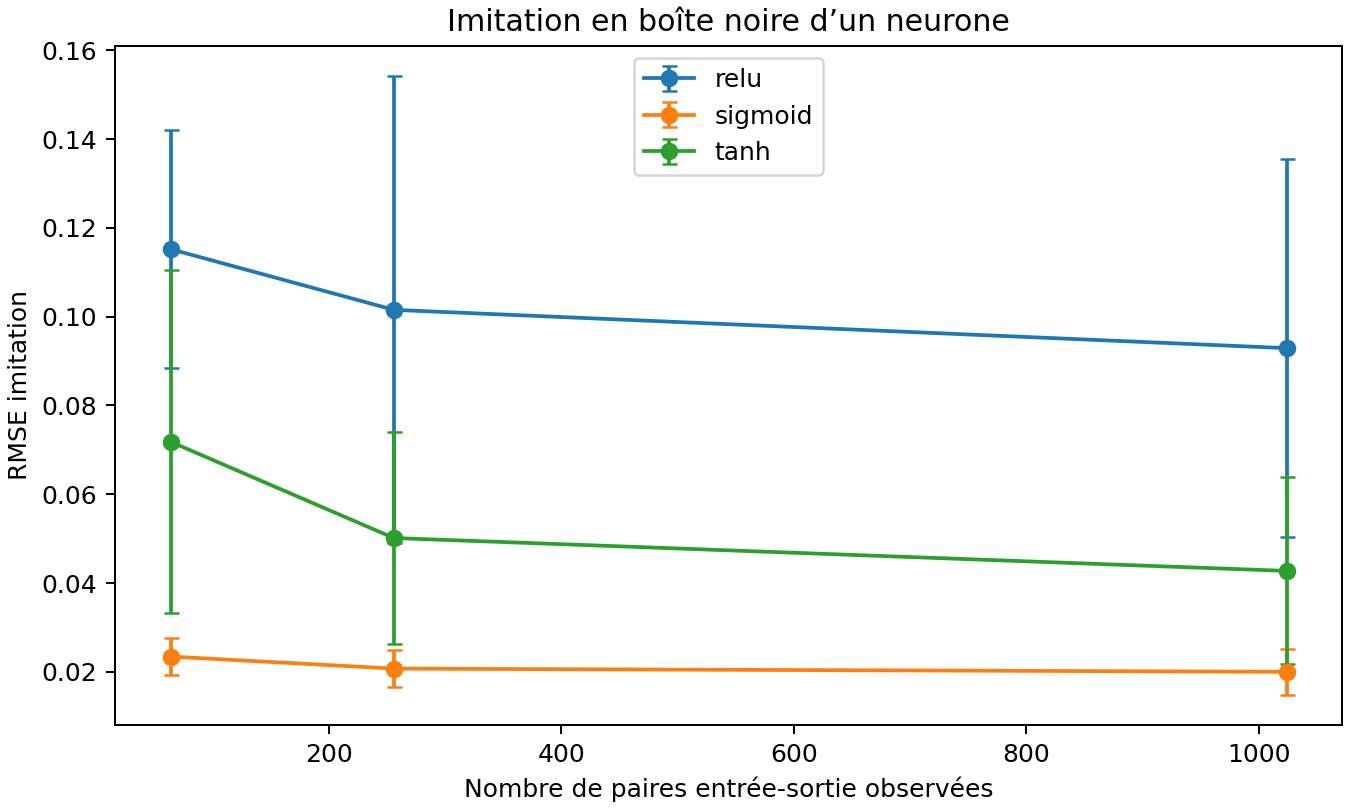
\includegraphics[width=.78\textwidth]{imitation_neurone_budget.png}
\caption{Fidélité d'imitation selon le nombre de paires entrée-sortie autorisées.}\label{fig:imitation}
\end{figure}

Sur 256 observations, le RMSE moyen entre cibles vaut environ 0.102 sur ReLU, 0.021 sur sigmoïde et 0.050 sur tanh. Le score $R^2$ est élevé sur la distribution tenue à part. Cela soutient H2 dans cette famille très restreinte : une sonde RBF peut approximer la fonction entrée-sortie de certains neurones simples à partir d'observations.

\subsection{Sensibilité au budget de paramètres — analyse exploratoire}
Le neurone cible affine+activation en dimension 2 n'a que trois paramètres continus ($w_1,w_2,b$). La sonde RBF à 20 centres a 81 paramètres ; le résultat primaire ne saurait donc être interprété comme une égalité de capacité.

\begin{table}[htbp]
\centering
\small
\setlength{\tabcolsep}{4pt}
\renewcommand{\arraystretch}{1.08}
\begin{tabular}{llrrr}
\toprule
Famille cible & Centres RBF & Paramètres sonde & RMSE & R$^2$ \\
\midrule
tanh & 1 & 5 & 0.2851 $\pm$ 0.1197 & 0.8433 $\pm$ 0.0743 \\
tanh & 2 & 9 & 0.1649 $\pm$ 0.0893 & 0.9474 $\pm$ 0.0364 \\
tanh & 4 & 17 & 0.1238 $\pm$ 0.0696 & 0.9699 $\pm$ 0.0222 \\
tanh & 8 & 33 & 0.0786 $\pm$ 0.0505 & 0.9875 $\pm$ 0.0106 \\
tanh & 20 & 81 & 0.0501 $\pm$ 0.0264 & 0.9951 $\pm$ 0.0031 \\
relu & 1 & 5 & 0.6888 $\pm$ 0.3785 & 0.6544 $\pm$ 0.0858 \\
relu & 2 & 9 & 0.5260 $\pm$ 0.3382 & 0.8008 $\pm$ 0.0917 \\
relu & 4 & 17 & 0.3109 $\pm$ 0.1426 & 0.9256 $\pm$ 0.0145 \\
relu & 8 & 33 & 0.1837 $\pm$ 0.0943 & 0.9745 $\pm$ 0.0054 \\
relu & 20 & 81 & 0.1015 $\pm$ 0.0599 & 0.9926 $\pm$ 0.0024 \\
sigmoid & 1 & 5 & 0.1048 $\pm$ 0.0443 & 0.8004 $\pm$ 0.1331 \\
sigmoid & 2 & 9 & 0.0674 $\pm$ 0.0253 & 0.9081 $\pm$ 0.0678 \\
sigmoid & 4 & 17 & 0.0473 $\pm$ 0.0144 & 0.9467 $\pm$ 0.0529 \\
sigmoid & 8 & 33 & 0.0327 $\pm$ 0.0079 & 0.9680 $\pm$ 0.0379 \\
sigmoid & 20 & 81 & 0.0207 $\pm$ 0.0042 & 0.9869 $\pm$ 0.0161 \\
\bottomrule
\end{tabular}
\caption{Analyse secondaire de capacité à budget d'observation fixé à 256 paires. Un neurone cible affine+activation possède trois paramètres continus en 2D. Les sondes utilisent 5 à 81 paramètres selon le nombre de centres.}
\label{tab:parameterbudget}
\end{table}
\begin{figure}[htbp]\centering
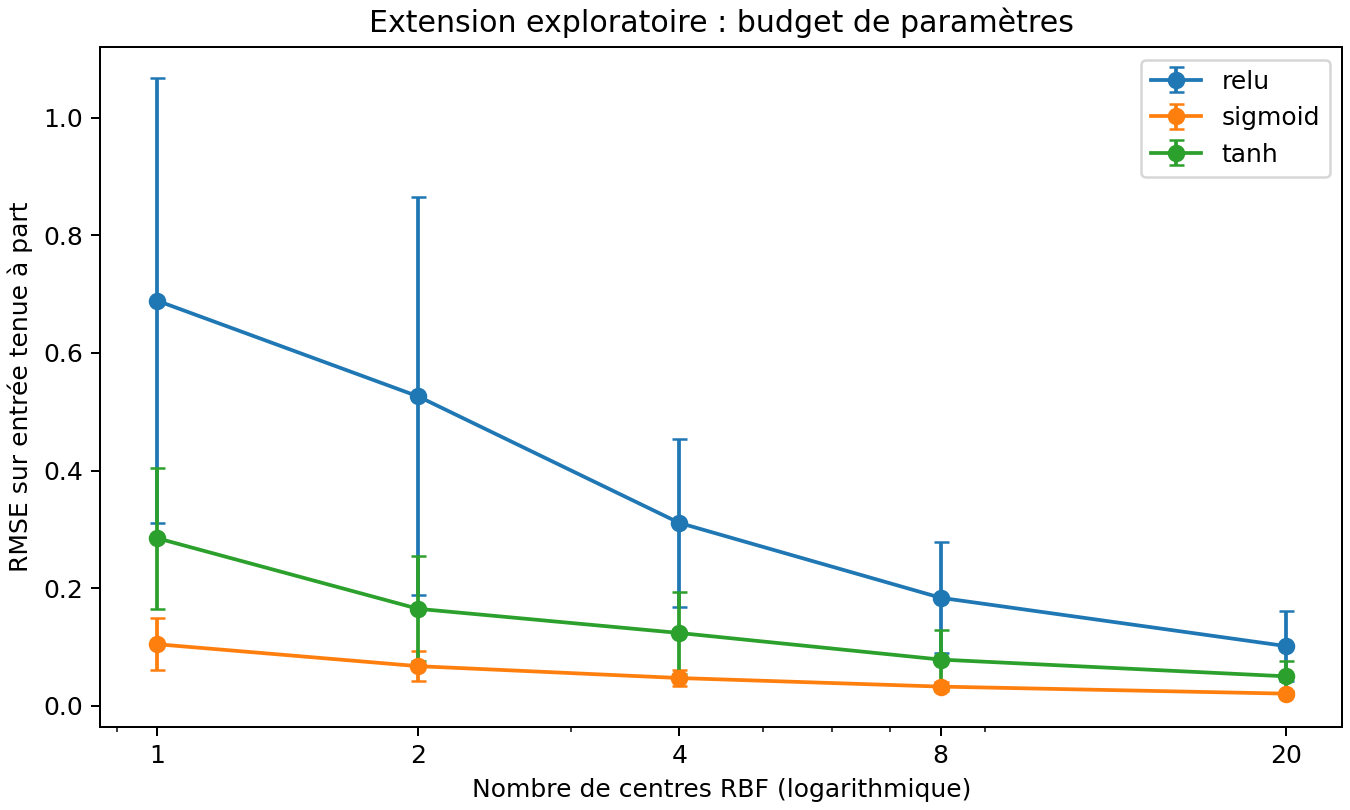
\includegraphics[width=.78\textwidth]{budget_parametres_imitation_exploratoire.png}
\caption{Analyse exploratoire : relation entre budget paramétrique de la sonde et erreur d'imitation.}\label{fig:budget}
\end{figure}

Le RMSE baisse généralement avec le nombre de centres, mais le coût en paramètres croît de 5 à 81. Avec un seul centre, $R^2$ est nettement moins élevé, notamment sur ReLU ; cette ablation rend explicite le rôle de capacité. Elle ne compare pas encore toutes les familles de sonde ni les modèles à budget exactement égal.

\subsection{Changement de distribution — analyse exploratoire}
Les sondes sont entraînées sur des entrées uniformes dans $[-2.5,2.5]^2$, puis évaluées sur une distribution translatée de $(+1.5,-1.5)$, sans réentraînement.

\begin{table}[htbp]
\centering
\small
\setlength{\tabcolsep}{4pt}
\renewcommand{\arraystretch}{1.08}
\begin{tabular}{llrrr}
\toprule
Famille cible & Paires & RMSE in-domain & RMSE entrée décalée & R$^2$ décalé \\
\midrule
tanh & 64 & 0.0718 & 0.1719 & 0.749 \\
tanh & 256 & 0.0501 & 0.2173 & 0.540 \\
tanh & 1024 & 0.0427 & 0.1792 & 0.732 \\
relu & 64 & 0.1152 & 0.8308 & 0.260 \\
relu & 256 & 0.1015 & 0.7651 & 0.317 \\
relu & 1024 & 0.0929 & 0.7149 & 0.183 \\
sigmoid & 64 & 0.0234 & 0.1659 & -0.320 \\
sigmoid & 256 & 0.0207 & 0.1544 & 0.091 \\
sigmoid & 1024 & 0.0200 & 0.1386 & 0.271 \\
\bottomrule
\end{tabular}
\caption{Analyse secondaire exploratoire. La distribution d'évaluation est translatée de (+1.5, -1.5), sans réentraînement ni choix d'hyperparamètres sur ces entrées.}
\label{tab:shift}
\end{table}
\begin{figure}[htbp]\centering
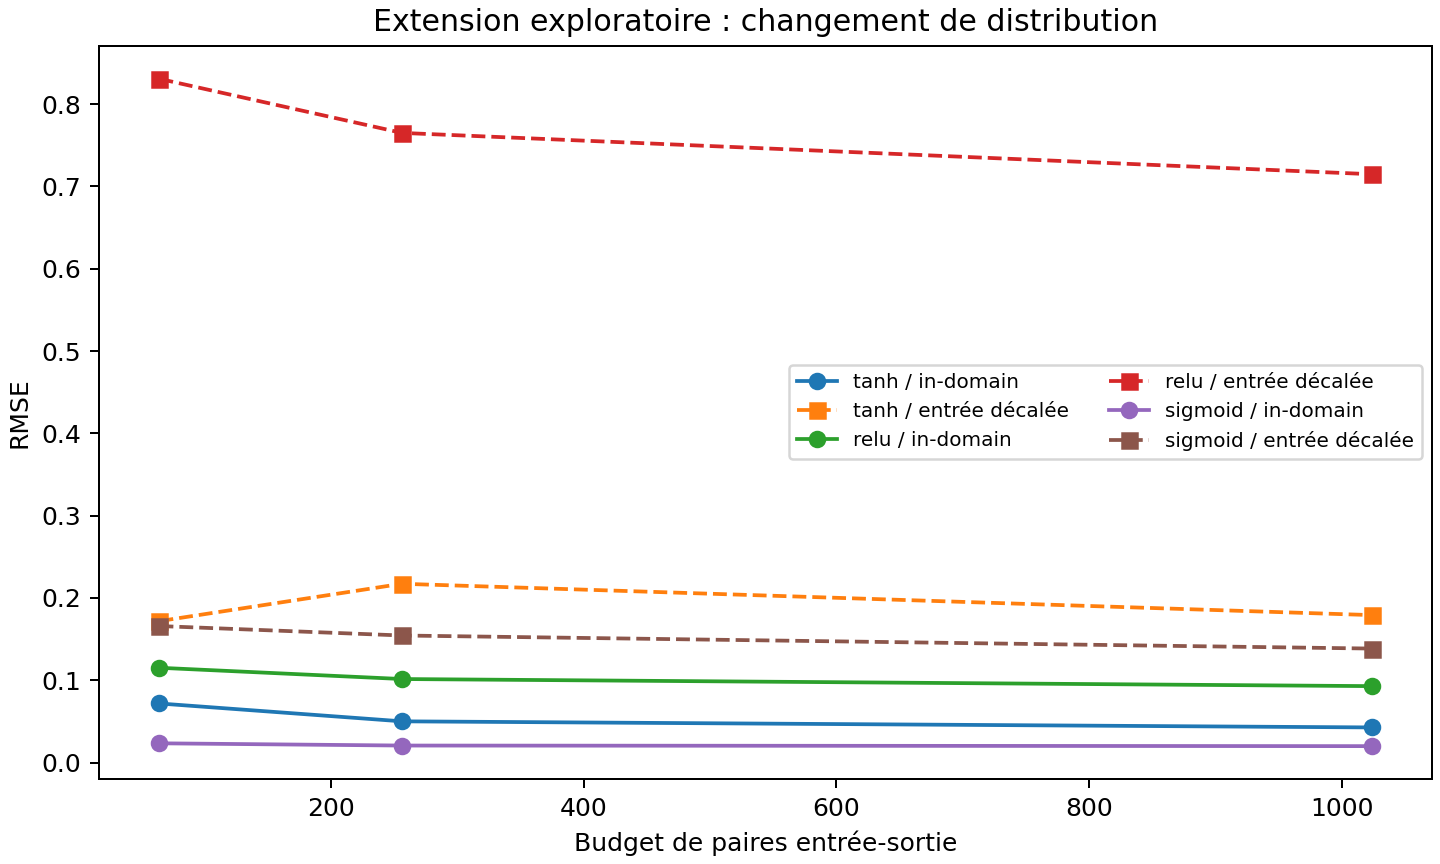
\includegraphics[width=.78\textwidth]{robustesse_changement_distribution_exploratoire.png}
\caption{Analyse exploratoire de généralisation sous un décalage de distribution.}\label{fig:shift}
\end{figure}

Le RMSE augmente fortement hors distribution. Pour ReLU, il passe approximativement de 0.093 à 0.715 avec 1024 observations ; pour tanh, de 0.043 à 0.179 ; pour sigmoïde, de 0.020 à 0.139. H3 n'est donc pas soutenue comme propriété générale : une bonne fidélité in-domain ne garantit pas une bonne extrapolation.

\section{Résultats 3 — Remplacement et composition}
La composition est testée sur deux lunes et le benchmark de diagnostic. Un MLP source à 16 unités cachées est entraîné sur le sous-ensemble train. Pour chaque unité cachée, une sonde scalaire reçoit les paires entrée/activation observée sur train. À l'évaluation, les activations des premières unités sont substituées par les prédictions des sondes, tandis que le lecteur de sortie original est gardé.

\begin{table}[htbp]
\centering
\small
\setlength{\tabcolsep}{4pt}
\renewcommand{\arraystretch}{1.08}
\begin{tabular}{lrrr}
\toprule
Tâche & MAE activation & RMSE activation & R$^2$ activation \\
\midrule
Deux lunes & 0.0531 $\pm$ 0.0089 & 0.0694 $\pm$ 0.0108 & 0.9820 $\pm$ 0.0043 \\
Cancer du sein (benchmark) & 0.2478 $\pm$ 0.0194 & 0.3153 $\pm$ 0.0239 & 0.8654 $\pm$ 0.0257 \\
\bottomrule
\end{tabular}
\caption{Fidélité de 16 sondes RBF sur les activations cachées du MLP, moyenne sur neurones puis sur trois graines. Les sondes ont 49 paramètres chacun en 2D et 257 en 30D ; un neurone du MLP a 3 paramètres d'entrée pour la tâche 2D ou 31 en 30D.}
\label{tab:fidelite}
\end{table}
\begin{table}[htbp]
\centering
\scriptsize
\setlength{\tabcolsep}{4pt}
\renewcommand{\arraystretch}{1.08}
\begin{tabular}{llrrr}
\toprule
Tâche & Unités & MLP exact. \% & Après \% & Écart logits \\
\midrule
Deux lunes & 1 & 92.87 $\pm$ 2.05 & 92.96 $\pm$ 1.89 & 0.016 $\pm$ 0.001 \\
Deux lunes & 4 & 92.87 $\pm$ 2.05 & 92.41 $\pm$ 1.85 & 0.089 $\pm$ 0.051 \\
Deux lunes & 16 & 92.87 $\pm$ 2.05 & 88.52 $\pm$ 1.43 & 0.469 $\pm$ 0.164 \\
Cancer du sein (benchmark) & 1 & 97.66 $\pm$ 1.01 & 97.95 $\pm$ 0.51 & 0.133 $\pm$ 0.025 \\
Cancer du sein (benchmark) & 4 & 97.66 $\pm$ 1.01 & 98.25 $\pm$ 0.88 & 0.454 $\pm$ 0.046 \\
Cancer du sein (benchmark) & 16 & 97.66 $\pm$ 1.01 & 98.83 $\pm$ 1.01 & 1.596 $\pm$ 0.042 \\
\bottomrule
\end{tabular}
\caption{Substitution de composants. La lecture de sortie du MLP enseignant est conservée. La différence de logits est une mesure de fidélité comportementale ; l'exactitude peut rester stable malgré cette différence.}
\label{tab:composition}
\end{table}
\begin{figure}[htbp]\centering
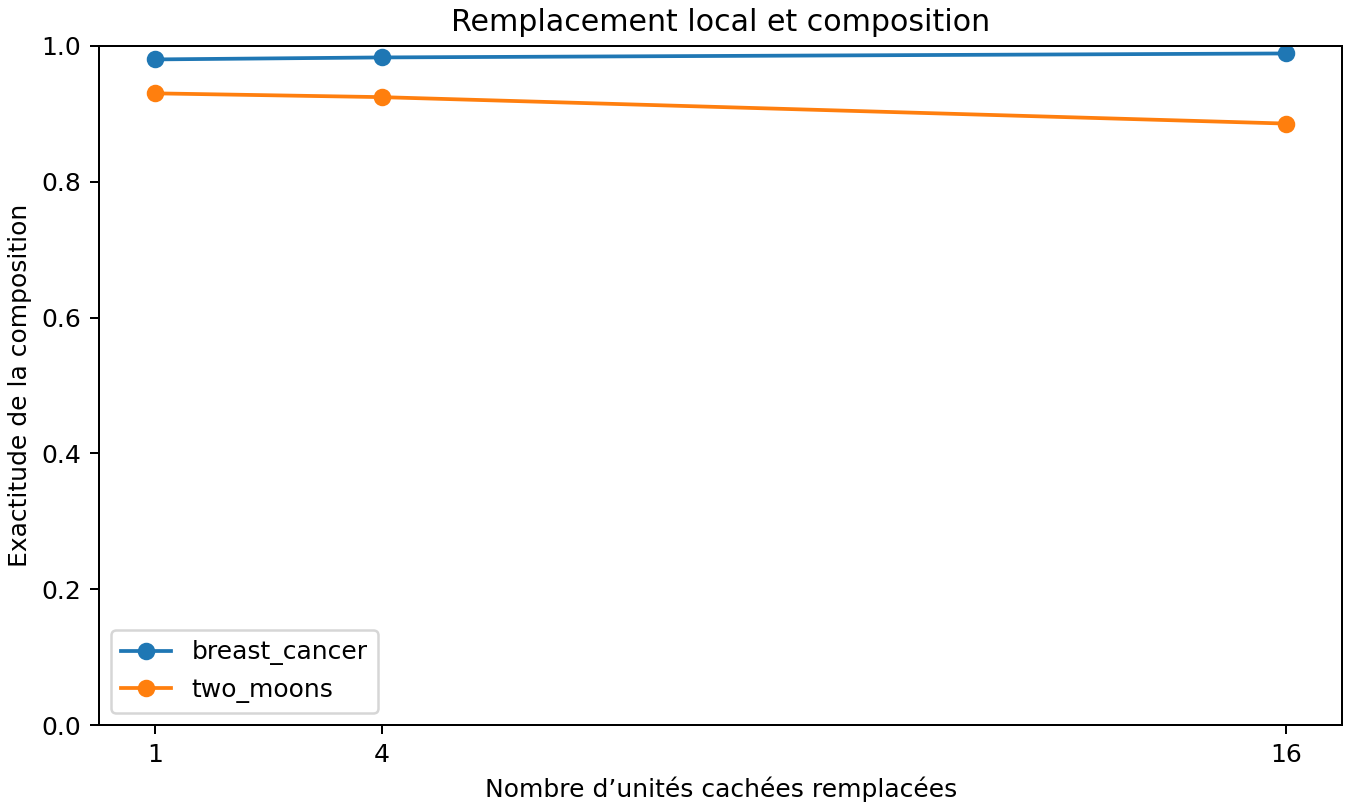
\includegraphics[width=.78\textwidth]{composition_remplacement.png}
\caption{Exactitude après remplacement de 1, 4 ou 16 unités cachées dans la composition. La variation des logits est rapportée séparément.}\label{fig:composition}
\end{figure}

La composition v1.2 utilise les graines prévues 411/522/633. Sur deux lunes, la précision moyenne du MLP enseignant est 92.87\% ; le remplacement de 1, 4 et 16 unités donne respectivement 92.96\%, 92.41\% et 88.52\%, avec un écart absolu moyen de logits de 0.016, 0.089 et 0.469. Sur le benchmark public, la précision enseignante est 97.66\% et le remplacement de 1, 4 et 16 unités donne 97.95\%, 98.25\% et 98.83\%, alors que l'écart moyen de logits croît de 0.133 à 0.454 puis 1.596. Cette divergence montre que l'exactitude de classe peut masquer une fidélité réduite au système source. Le nombre d'unités remplacées constitue une intervention de composition contrôlée.

La composition conserve le lecteur de sortie original ; elle n'est donc pas un étudiant autonome. La conclusion correcte est plus étroite : des sondes peuvent remplacer certains composants localement, mais les erreurs changent la sortie composée et s'accumulent. H4 n'est que partiellement soutenue et dépend de la tâche et de la métrique.

\section{Résultats 4 — Contrôle de budget final égal (exploratoire)}
B bénéficie dans l'analyse principale de 700 époques finales, contre 220 pour A et le MLP. Le tableau suivant compare les modèles après 700 époques finales ; B conserve le coût de 35 étapes d'hypergradient en amont. Il s'agit d'un contrôle exploratoire, pas d'une égalité totale de temps de calcul.

\begin{table}[htbp]
\centering
\small
\setlength{\tabcolsep}{4pt}
\renewcommand{\arraystretch}{1.08}
\begin{tabular}{llrrr}
\toprule
Tâche & Méthode & Exactitude \% & ROC-AUC & Log-loss \\
\midrule
Deux lunes & RBF adaptative & 95.74 $\pm$ 0.58 & 0.9894 $\pm$ 0.0031 & 0.130 $\pm$ 0.009 \\
Deux lunes & RBF règle/taux appris & 95.74 $\pm$ 0.58 & 0.9899 $\pm$ 0.0031 & 0.127 $\pm$ 0.010 \\
Deux lunes & RBF fixe & 86.94 $\pm$ 1.44 & 0.9335 $\pm$ 0.0084 & 0.332 $\pm$ 0.016 \\
Deux lunes & MLP & 95.65 $\pm$ 0.70 & 0.9895 $\pm$ 0.0027 & 0.129 $\pm$ 0.008 \\
Cercles & RBF adaptative & 94.35 $\pm$ 0.89 & 0.9894 $\pm$ 0.0030 & 0.132 $\pm$ 0.017 \\
Cercles & RBF règle/taux appris & 94.72 $\pm$ 1.11 & 0.9901 $\pm$ 0.0034 & 0.130 $\pm$ 0.020 \\
Cercles & RBF fixe & 92.96 $\pm$ 0.42 & 0.9851 $\pm$ 0.0015 & 0.235 $\pm$ 0.021 \\
Cercles & MLP & 94.35 $\pm$ 0.98 & 0.9884 $\pm$ 0.0031 & 0.139 $\pm$ 0.019 \\
Produit/XOR bruité & RBF adaptative & 93.43 $\pm$ 0.70 & 0.9478 $\pm$ 0.0033 & 0.275 $\pm$ 0.010 \\
Produit/XOR bruité & RBF règle/taux appris & 93.80 $\pm$ 1.12 & 0.9487 $\pm$ 0.0016 & 0.280 $\pm$ 0.008 \\
Produit/XOR bruité & RBF fixe & 93.06 $\pm$ 0.00 & 0.9498 $\pm$ 0.0026 & 0.335 $\pm$ 0.001 \\
Produit/XOR bruité & MLP & 94.35 $\pm$ 0.16 & 0.9464 $\pm$ 0.0031 & 0.244 $\pm$ 0.003 \\
Cancer du sein (benchmark) & RBF adaptative & 98.25 $\pm$ 0.88 & 0.9947 $\pm$ 0.0078 & 0.093 $\pm$ 0.033 \\
Cancer du sein (benchmark) & RBF règle/taux appris & 98.25 $\pm$ 0.88 & 0.9947 $\pm$ 0.0078 & 0.088 $\pm$ 0.034 \\
Cancer du sein (benchmark) & RBF fixe & 94.15 $\pm$ 1.34 & 0.9890 $\pm$ 0.0062 & 0.156 $\pm$ 0.026 \\
Cancer du sein (benchmark) & MLP & 96.78 $\pm$ 0.51 & 0.9891 $\pm$ 0.0099 & 0.124 $\pm$ 0.079 \\
\bottomrule
\end{tabular}
\caption{Analyse secondaire exploratoire : tous les modèles reçoivent 700 époques finales. B conserve en plus 35 étapes de méta-ajustement. Ce tableau teste si l'écart principal dépend seulement des époques ; il ne constitue pas un contrôle strict à budget total de calcul égal.}
\label{tab:equalepochs}
\end{table}

Sous 700 époques finales, A et B sont très proches sur le benchmark réel (environ 98.25\% tous les deux), sur deux lunes (95.74\% tous les deux), sur les cercles (94.35\% contre 94.72\%) et sur le produit/XOR (93.43\% contre 93.80\%). Le bénéfice apparent de B dans la comparaison principale se réduit donc une fois le nombre d'époques d'A augmenté. Il ne faut pas attribuer l'écart principal au seul fait que le mécanisme de sonde aurait été « appris ».

\section{Complément préenregistré -- cas réel multiclasse plus exigeant}
Le benchmark binaire de diagnostic public de l'expérience primaire est réel mais petit. Pour tester le protocole sur un cas d'usage réel plus riche, un complément distinct a été préenregistré avant exécution. Il utilise le jeu public de chiffres manuscrits de scikit-learn : 1 797 images 8×8, 64 entrées par image et dix classes. Les partitions sont les graines 1428, 2539 et 3640, stratifiées en 60/20/20 ; le standardiseur est ajusté sur train seulement. Ce jeu est un benchmark de laboratoire compact, non une validation de reconnaissance d'écriture en production.

\begin{table}[htbp]
\centering
\scriptsize
\setlength{\tabcolsep}{3.6pt}
\renewcommand{\arraystretch}{1.08}
\begin{tabular}{llrrrr}
\toprule
Méthode & Exactitude (\%) & Balanced acc. (\%) & F1 macro (\%) & Log-loss & Param. \\
\midrule
Sonde RBF fixe & 76.67 $\pm$ 3.38 & 76.66 $\pm$ 3.38 & 76.48 $\pm$ 3.37 & 1.304 $\pm$ 0.004 & 170 \\
Sonde RBF adaptative & 87.31 $\pm$ 3.52 & 87.34 $\pm$ 3.49 & 87.34 $\pm$ 3.45 & 0.752 $\pm$ 0.055 & 1210 \\
Sonde à mécanisme partiellement appris & 78.33 $\pm$ 2.27 & 78.28 $\pm$ 2.22 & 78.00 $\pm$ 2.11 & 1.419 $\pm$ 0.026 & 1210 \\
MLP de référence & 96.76 $\pm$ 1.16 & 96.77 $\pm$ 1.16 & 96.77 $\pm$ 1.16 & 0.126 $\pm$ 0.032 & 1210 \\
\bottomrule
\end{tabular}
\caption{Reconnaissance réelle de chiffres manuscrits à dix classes : images 8×8, 64 entrées, trois partitions prédéfinies. Moyenne $\pm$ écart-type sur trois graines. A, B et le MLP disposent chacun de 1 210 paramètres entraînables ; le contrôle RBF fixe de 170.}
\label{tab:digits_class}
\end{table}
\begin{figure}[htbp]\centering
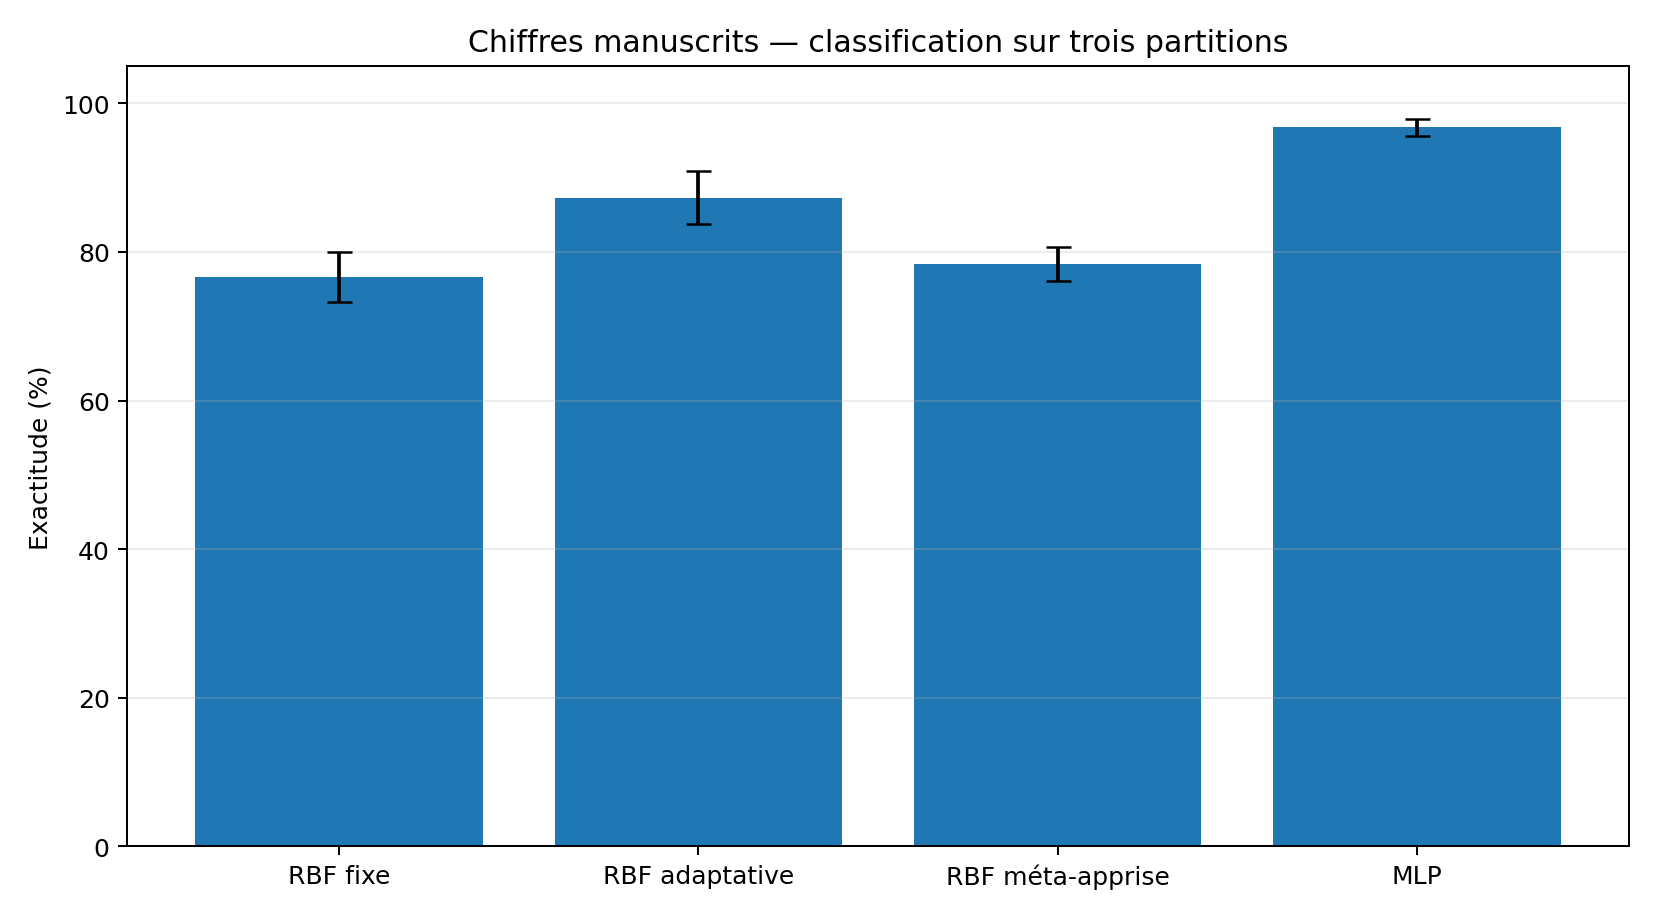
\includegraphics[width=.83\textwidth]{digits_comparaison_classification.png}
\caption{Exactitude des quatre méthodes sur le benchmark réel à dix classes ; les barres d'erreur indiquent l'écart-type sur trois partitions.}\label{fig:digits_class}
\end{figure}

Sur ces trois partitions, la RBF adaptative A atteint 87.31\% d'exactitude moyenne ; la variante B dont les taux de mise à jour sont méta-appris atteint 78.33\% ; la RBF fixe atteint 76.67\% ; le MLP avec capacité paramétrique égale à A/B (1 210 paramètres chacun) atteint 96.76\%. Sur ce cas réel multiclasse, le mécanisme d'adaptation méta-appris ne donne donc pas de gain observé : B est nettement moins performante que A et que le MLP. Ce résultat négatif est conservé sans ajustement a posteriori. Trois partitions seulement imposent une incertitude importante.

\begin{table}[htbp]
\centering
\scriptsize
\setlength{\tabcolsep}{3.6pt}
\renewcommand{\arraystretch}{1.08}
\begin{tabular}{lrrrrr}
\toprule
Unités remplacées & MLP source (\%) & Composé (\%) & Accord source (\%) & RMSE logits & Écart prob. \\
\midrule
1 & 96.76 $\pm$ 1.16 & 96.11 $\pm$ 1.00 & 99.17 $\pm$ 0.00 & 0.389 $\pm$ 0.023 & 0.0033 $\pm$ 0.0005 \\
4 & 96.76 $\pm$ 1.16 & 95.74 $\pm$ 1.28 & 98.15 $\pm$ 1.05 & 0.783 $\pm$ 0.022 & 0.0084 $\pm$ 0.0012 \\
16 & 96.76 $\pm$ 1.16 & 86.57 $\pm$ 1.95 & 86.94 $\pm$ 2.82 & 1.878 $\pm$ 0.023 & 0.0547 $\pm$ 0.0027 \\
\bottomrule
\end{tabular}
\caption{Substitution de 1, 4 ou 16 unités cachées sur la reconnaissance manuscrite. Le lecteur de sortie du MLP source est conservé ; il ne s’agit pas d’un modèle étudiant autonome. Moyenne $\pm$ écart-type sur trois partitions.}
\label{tab:digits_comp}
\end{table}
\begin{figure}[htbp]\centering
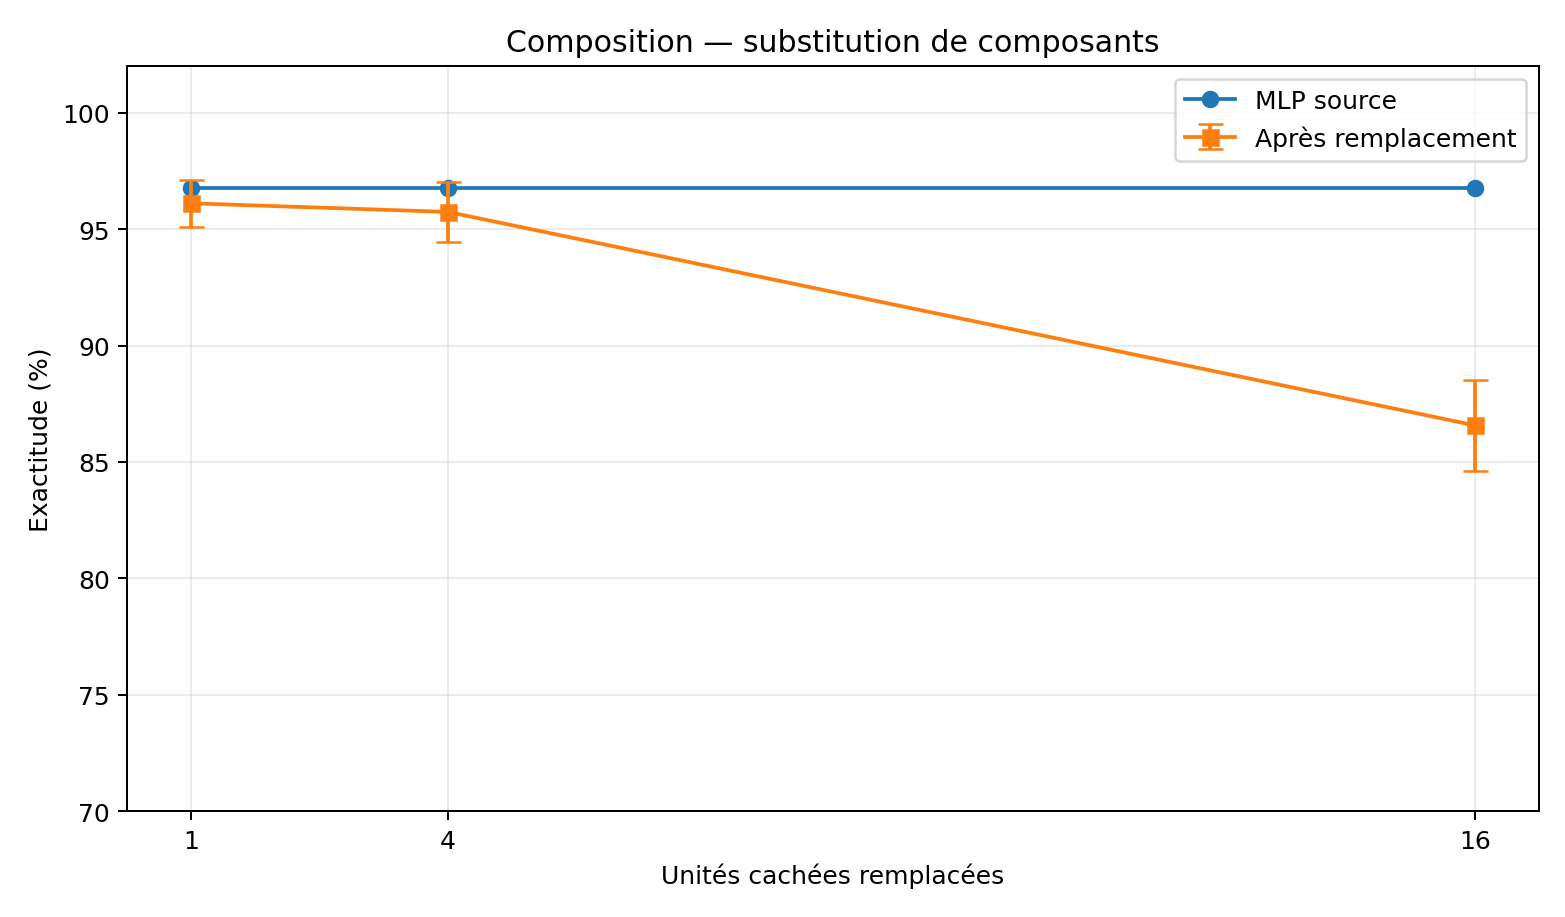
\includegraphics[width=.82\textwidth]{digits_composition_remplacement.png}
\caption{Exactitude du MLP source et du système après remplacement d'unités cachées.}\label{fig:digits_comp}
\end{figure}
\begin{figure}[htbp]\centering
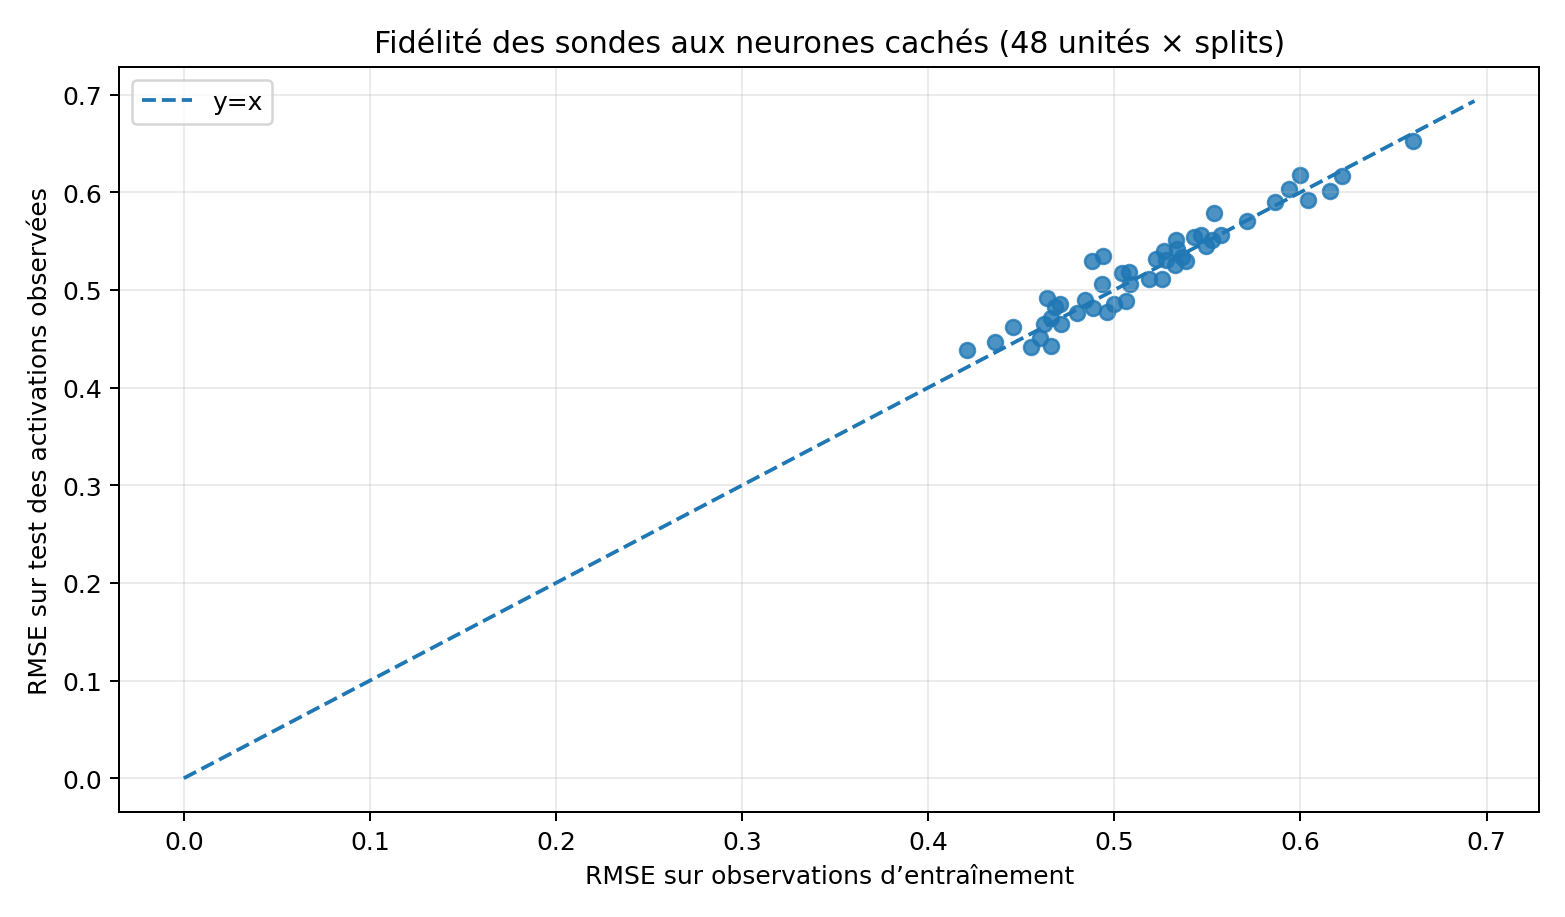
\includegraphics[width=.82\textwidth]{digits_fidelite_activations.png}
\caption{RMSE sur les activations de train et de test pour les 48 sondes imitant les unités cachées.}\label{fig:digits_fidelity}
\end{figure}

La fidélité des sondes scalaires aux activations cachées du MLP a un RMSE moyen de 0.5218 au test (RMSE d'entraînement moyen 0.5184). Chaque sonde utilisée pour imiter une unité cachée comporte 529 paramètres entraînables, alors qu'une unité cachée du MLP 64→16 possède 65 paramètres affines. La sonde a donc un budget de paramètres nettement supérieur ; ces résultats ne montrent pas une équivalence à capacité égale.

Le remplacement d'une ou quatre unités conserve une exactitude proche de celle de la source, mais l'écart des logits augmente. Le remplacement des 16 unités fait baisser l'exactitude composée moyenne à 86.57\%, contre 96.76\% pour le MLP source, et l'accord des classes source/composé à 86.94\%. Les erreurs locales peuvent donc s'accumuler lors de la composition. Le lecteur de sortie original est maintenu : il ne s'agit pas d'une reconstruction autonome.

Les prédictions gelées, matrices de confusion par méthode/split, fidélités par unité, intervalles t descriptifs à 95\% (\texttt{digits\_synthese\_intervalles\_95.csv} et \texttt{digits\_composition\_intervalles\_95.csv}), registre des partitions et empreintes sont fournis dans les CSV et JSON associés. Les labels du test ne sont pas des arguments des fonctions d'entraînement.

\section{Hypothèses : verdicts circonscrits}
\begin{description}[leftmargin=1.3cm,style=nextline]
\item[H1 — Apprentissage de tâche :] soutenue dans les tâches testées, mais avec des performances variables selon le domaine : sur les chiffres manuscrits, la RBF adaptative reste sous le MLP. Le contrôle fixe est plus faible, mais son budget de paramètres est moindre.
\item[H2 — Imitation de neurones :] soutenue pour une famille artificielle limitée de neurones scalaires, grâce à des exemples entrée-sortie autorisés, dans le domaine in-domain testé.
\item[H3 — Généralisation :] soutenue partiellement sur une partition iid tenue à part ; contredite comme affirmation robuste sous le décalage d'entrée exploratoire. Les interventions plus générales ne sont pas couvertes.
\item[H4 — Composition :] partiellement soutenue. Le remplacement local est réalisable, mais la fidélité de logits décroît nettement quand plus d'unités sont remplacées, et l'exactitude finale dépend de la tâche.
\item[H5 — Généralité :] non établie. Cinq tâches de classification, dont trois synthétiques et deux benchmarks réels compacts, et trois partitions par tâche constituent un échantillon limité.
\item[H6 — Neurone cas particulier de sonde :] les résultats sont compatibles avec une interprétation opérationnelle et une capacité d'approximation ; ils ne démontrent pas une équivalence mathématique universelle.
\end{description}

\section{Limites scientifiques et intégrité}
\begin{enumerate}[leftmargin=1.15cm]
\item \textbf{Capacité.} Les sondes d'imitation à 20 centres sont beaucoup plus paramétriques que le neurone isolé ; l'analyse exploratoire confirme que le nombre de paramètres contribue au score.
\item \textbf{Famille d'activation.} L'expérience boîte noire ne couvre que trois activations simples et des cibles affines en deux dimensions. Cela ne représente pas toutes les unités modernes, les normalisations, les états contextuels ou les dynamiques temporelles.
\item \textbf{Méca­nisme appris.} La condition B apprend des taux par groupe ; elle conserve la RBF et le type de mise à jour prédéfinis. Ce n'est pas un optimiseur découvert de novo. Les hypergradients utilisent la validation autorisée.
\item \textbf{Comparabilité du calcul.} Les époques principales de B sont plus nombreuses que celles d'A/D ; le contrôle 700 époques est présenté séparément et montre que l'avantage se réduit.
\item \textbf{Compositions.} Le lecteur de sortie source est conservé. Nous ne démontrons donc pas un modèle autonome complet construit uniquement par sondes.
\item \textbf{Données réelles.} Les deux benchmarks réels sont compacts : le jeu de diagnostic n’est pas une validation clinique et les chiffres manuscrits ne sont pas un test de reconnaissance en production.
\item \textbf{Statistique.} Trois partitions/graines imposent une incertitude importante. Les intervalles t fournis sont descriptifs ; ils ne prouvent ni une supériorité générale ni une réplication indépendante multi-site.
\item \textbf{Anti-triche.} Les interfaces d'ajustement n'acceptent pas les labels de test ni les paramètres cibles, les graines d'imitation sont indépendantes et les hachages des lignes sont disjoints dans chaque partition. L'audit ne garantit pas contre tout canal covert possible dans un même environnement local.
\item \textbf{Préenregistrement.} Les résultats primaires utilisent le protocole v1.1 gelé avant exécution ; la composition suit le correctif v1.2 gelé avant relance ; la reconnaissance de chiffres suit un protocole complémentaire gelé avant son exécution. Les essais de mise au point antérieurs sont exclus. Les analyses de budget de paramètres, décalage d'entrée et époques égales sont explicitement exploratoires et postérieures au résultat primaire.
\item \textbf{Traçabilité administrative.} Le finaliseur utilisé pour les agrégats et le manifeste a été retouché après l'exécution pour séparer les graines de classification et de composition. Son empreinte actuelle diffère de l'empreinte pré-exécution ; cette divergence est décrite dans le journal d'audit. Le code d'entraînement et le lanceur de composition restent conformes aux empreintes gelées.
\end{enumerate}

\section{Reproductibilité et artefacts}
Le pipeline est CPU-only et utilise Python, PyTorch, NumPy, pandas, scikit-learn, SciPy et Matplotlib. Les données synthétiques sont générées par scripts ; le jeu réel est obtenu par la fonction de chargement standard du jeu de données de scikit-learn. Les prédictions d'évaluation sont enregistrées dans \texttt{predictions\_test\_apres\_gel.csv} après gel du modèle.

L'audit final est \texttt{PASS\_WITH\_LIMITATIONS}, avec 12 contrôles passés et une limitation de sandbox explicitement déclarée. Le registre d'intégrité et les empreintes sont inclus dans l'archive.

Commandes détaillées de reproduction, versions et limitations sont dans \texttt{README.md}. Les résultats par graine, intervalles, traces des cibles, métriques par neurone et compositions sont fournis en CSV et JSON ; l'archive de reproductibilité contient aussi le code et les deux documents source utilisés.

\section{Conclusion finale}
Cette expérience apporte des résultats empiriques ciblés : une famille de sondes adaptatives peut apprendre certaines tâches, imiter par observation certains neurones artificiels simples et être insérée à leur place dans des compositions. Le complément réel multiclasse montre cependant que la RBF adaptative reste nettement derrière le MLP sur les chiffres manuscrits, et que la variante à mécanisme partiellement appris peut être moins efficace que la sonde standard. Les résultats favorisent l'idée qu'un neurone peut être étudié opérationnellement comme composant observable et qu'une sonde peut en approximer le comportement sous contraintes.

Ils ne démontrent pas que le neurone est universellement un cas particulier de sonde, que chaque sonde peut apprendre le fonctionnement de chaque neurone, ni qu'une composition de sondes remplace exactement un système complet. La fidélité dépend du budget de paramètres, des données d'observation, du domaine et de la profondeur de composition. La prochaine preuve la plus décisive serait une expérience à budget strictement égal, sur une classe de neurones plus large, avec test shifté pré-enregistré et remplacement autonome de tous les composants sans conserver de lecteur source.

\end{document}
